\subsection{Technical overview}
The basic tool of our algorithms is a clustering algorithm in \cite{bodwin2021better}. Let $G = (V, E)$ be the input undirected unweighted graph. Roughly speaking, for any radius parameter $R$, we can decompose the graph into a set $\bset$ of balls that may share vertices, with the following properties.
\begin{itemize}
	\item (Radius) The radius of each ball in $\bset$ is roughly $R$.
	\item (Coverage) The union of all balls in $\bset$ covers the whole graph $G$.
	\item (Disjointness) The total size of the balls in $\bset$ is linear in $n$.
\end{itemize}

Next, we will describe how to utilize the above clustering to construct new sublinear additive spanners and additive spanners, respectively.

\subsubsection{Sublinear additive spanners}

Our starting point is a spanner with stretch function $f(d) = d + O(d^{1/2})$ and $\tilde{O}(n^{8/7})$ edges, which improves upon the previous sparsity bound of $\tilde{O}(n^{20/17})$ in \cite{chechik2013new}. Consider any pair of vertices $s, t\in V$, and let $\pi$ be a shortest path between them of length $D$. We apply the clustering algorithm from \cite{bodwin2021better} with radius parameter $R = D^{1/2}$ to $G$, and obtain a set $\bset$ of balls. Intuitively, by the coverage property, and recalling that every ball in $\balls$ has radius roughly $R=D^{1/2}$, we can choose a subset of $O(D / R) = O(D^{1/2})$ balls from $\bset$ whose union contains the entire shortest path $\pi$.
%and furthermore, since the radius of each ball is $\Theta(R)$, intuitively we can prove that the total number of these balls is bounded by $O(D / R) = O(D^{1/2})$. 
See Figure \ref{overview-path-partition} for an illustration.

\begin{figure}[h]
	\begin{center}
		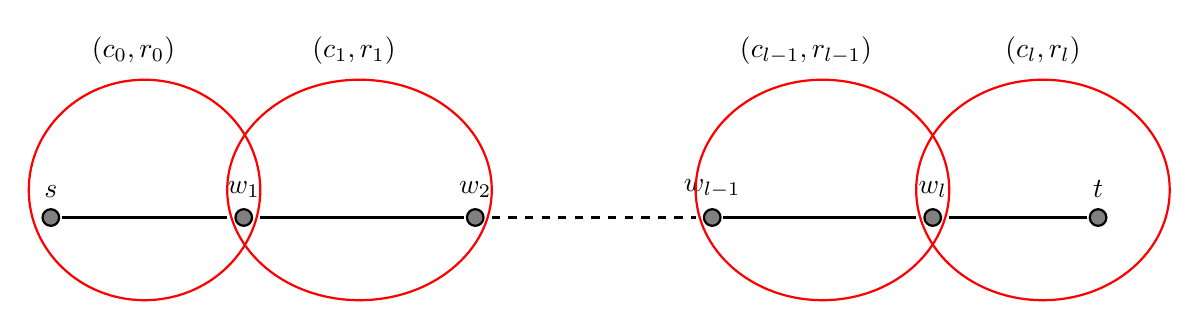
\begin{tikzpicture}[thick,scale=0.7]
	\draw (0, 0) node[circle, draw, fill=black!50, inner sep=0pt, minimum width=6pt, label = $s$] {};
	\draw (19, 0) node[circle, draw, fill=black!50, inner sep=0pt, minimum width=6pt,label = $t$] {};
	
	\draw (3.5, 0) node[circle, draw, fill=black!50, inner sep=0pt, minimum width=6pt,label = $w_1$] {};
	\draw [line width = 0.5mm] (0.2, 0) -- (3.2, 0);
	\draw [red] (1.7, 0.5) ellipse (2.1 and 2);
	\draw (1.5, 2.4) node[red, label={$\ball(c_0, r_{0})$}]{};
	
	\draw (7.7, 0) node[circle, draw, fill=black!50, inner sep=0pt, minimum width=6pt,label = $w_2$] {};
	\draw [line width = 0.5mm] (3.8, 0) -- (7.5, 0);
	\draw [red] (5.6, 0.5) ellipse (2.4 and 2);
	\draw (5.5, 2.4) node[red, label={$\ball(c_1, r_{1})$}]{};
	
	\draw (16, 0) node[circle, draw, fill=black!50, inner sep=0pt, minimum width=6pt,label = $w_l$] {};
	\draw [line width = 0.5mm] (18.8, 0) -- (16.3, 0);
	\draw [red] (18, 0.5) ellipse (2.3 and 2);
	\draw (18, 2.4) node[red, label={$\ball(c_{l}, r_{l})$}]{};
	
	\draw (12, 0) node[circle, draw, fill=black!50, inner sep=0pt, minimum width=6pt,label = $w_{l-1}$] {};
	\draw [line width = 0.5mm] (15.7, 0) -- (12.2, 0);
	\draw [red] (14, 0.5) ellipse (2.3 and 2);
	\draw (13.7, 2.4) node[red, label={$\ball(c_{l-1}, r_{l-1})$}]{};
	
	\draw [dashed] (8, 0) -- (11.7, 0); 
\end{tikzpicture}
	\end{center}
	\caption{An illustration of a covering of a shortest path $\pi$ between $s, t$ with at most $l = O(D^{1/2})$ balls from $\bset$. For simplicity, we assume that, for each index $0\le i\le l-1$, the balls $\ball(c_i,r_i)$ and $\ball(c_{i+1},r_{i+1})$ share exactly one vertex of $\pi$, denoted by $w_{i+1}$. We denote $s = w_0$ and $t = w_{l+1}$.}\label{overview-path-partition}
\end{figure}

Following the notations in Figure \ref{overview-path-partition}, assume the sequence of balls divides the path into subpaths $\set{\pi[w_i, w_{i+1}]}_{0\le i\le l}$. In order to preserve the distance between $s, t$ in $G$, a simple approach is to plant, within each subgraph $G[\ball(c_i, r_i)]$, a $6$-additive spanner from \cite{baswana2010additive} with  $O(|\ball(c_i, r_i)|^{4/3})$ edges. Then for each $i$, $\dist_{H}(w_i, w_{i+1})\leq \dist_G(w_i, w_{i+1}) + 6$, so $\dist_H(s,t)-\dist_G(s,t)\le 6(l+1)=O(D^{1/2})$. If we further assume that each ball in $\balls$ contains at most $n^{3/7}$ vertices, then by the disjointness property, the union of all these $6$-additive spanners contains at most $\sum_{\ball(c, r)\in\bset}|\ball(c, r)|^{4/3} = O(n^{8/7})$ edges. So we only need to deal with large balls that contain more than $n^{3/7}$ vertices.

A natural approach to handling the large balls is taking a random subset $S\subseteq V$ of $10n^{4/7}\log n$ vertices that hits all large balls with high probability, and try preserving pairwise distances between vertices in $S$, as preserving distances among a subset is conceivably easier than the whole graph.
%One can imagine that preserving pairwise distances between vertices in $S$ is hopefully easier than preserving all-pairs distances in $V$ as $S$ has a sublinear size.
In fact, if this can be done, then the distance between all pairs $s, t\in V$ is also well-preserved. 
%\begin{itemize}[leftmargin=*]\item If all balls $\ball(c_i, r_i)$ have sizes smaller than $n^{3/7}$, then those $6$-additive spanners within them already suffice for a good stretch.
To see why this is true, assume for simplicity that $\ball(c_1, r_1)$ and $\ball(c_{l-1}, r_{l-1})$ are the first and the last large ball, respectively. Then, by construction of $S$, there exist $u\in \ball(c_1, r_1)\cap S$ and $v\in \ball(c_{l-1}, r_{l-1})\cap S$, and it is easy to verify using triangle inequality that the following path connecting $s$ to $t$ in $H$ has length at most $\dist_G(s,t)+O(R)$; the path is the concatenation of (see \Cref{overview-hitset} for an illustration):
	\begin{itemize}[leftmargin=*]
		\item a path from $s$ to $w_1$ in the $6$-additive spanner within subgraph $G[\ball(c_0, r_0)]$; and similarly a path from $t$ to $w_l$ in the $6$-additive spanner within subgraph $G[\ball(c_l, r_l)]$;
		\item a path from $w_1$ to $u$ of length at most $2R$, as we can afford to add to $H$ a breadth-first search tree of $G[\ball(c_1, r_1)]$ beforehand; similarly, a path from $w_l$ to $v$ of length at most $2R$; and
		\item the shortest path connecting $u, v$ in $H$.
	\end{itemize}

\begin{figure}[h]
	\begin{center}
		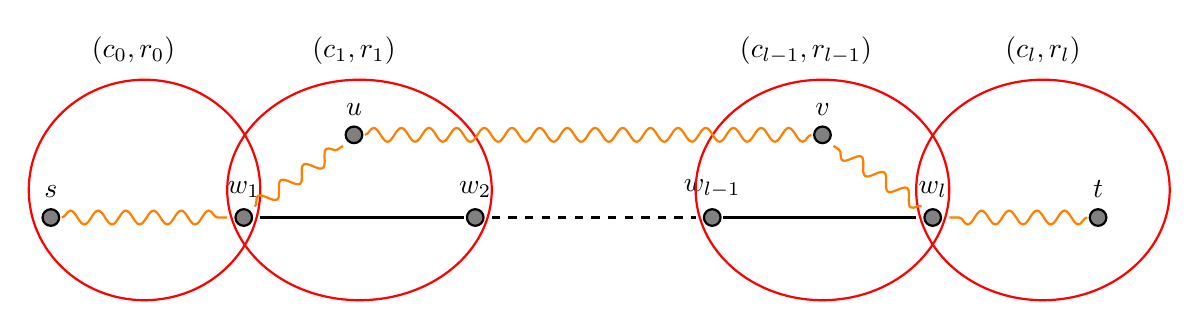
\begin{tikzpicture}[thick,scale=0.7]
	\draw (0, 0) node[circle, draw, fill=black!50, inner sep=0pt, minimum width=6pt, label = $s$] {};
	\draw (19, 0) node[circle, draw, fill=black!50, inner sep=0pt, minimum width=6pt,label = $t$] {};
	
	\draw (3.5, 0) node[circle, draw, fill=black!50, inner sep=0pt, minimum width=6pt,label = $w_1$] {};
	\draw [color=orange, style={decorate, decoration=snake}] (0.2, 0) -- (3.2, 0);
	\draw [red] (1.7, 0.5) ellipse (2.1 and 2);
	\draw (1.5, 2.4) node[red, label={$\ball(c_0, r_{0})$}]{};
	\draw (5.5, 1.5) node[circle, draw, fill=black!50, inner sep=0pt, minimum width=6pt,label = $u$] {};
	\draw [color=orange, style={decorate, decoration=snake}] (3.7, 0.2) -- (5.3, 1.3);
	
	\draw (7.7, 0) node[circle, draw, fill=black!50, inner sep=0pt, minimum width=6pt,label = $w_2$] {};
	\draw [line width = 0.5mm] (3.8, 0) -- (7.5, 0);
	\draw [red] (5.6, 0.5) ellipse (2.4 and 2);
	\draw (5.5, 2.4) node[red, label={$\ball(c_1, r_{1})$}]{};
	
	\draw (16, 0) node[circle, draw, fill=black!50, inner sep=0pt, minimum width=6pt,label = $w_l$] {};
	\draw [color=orange, style={decorate, decoration=snake}] (18.8, 0) -- (16.3, 0);
	\draw [red] (18, 0.5) ellipse (2.3 and 2);
	\draw (18, 2.4) node[red, label={$\ball(c_{l}, r_{l})$}]{};
	\draw (14, 1.5) node[circle, draw, fill=black!50, inner sep=0pt, minimum width=6pt,label = $v$] {};
	\draw [color=orange, style={decorate, decoration=snake}] (15.8, 0.2) -- (14.2, 1.3);
	
	\draw (12, 0) node[circle, draw, fill=black!50, inner sep=0pt, minimum width=6pt,label = $w_{l-1}$] {};
	\draw [line width = 0.5mm] (15.7, 0) -- (12.2, 0);
	\draw [red] (14, 0.5) ellipse (2.3 and 2);
	\draw (13.7, 2.4) node[red, label={$\ball(c_{l-1}, r_{l-1})$}]{};
	
	\draw [dashed] (8, 0) -- (11.7, 0);
	\draw [color=orange, style={decorate, decoration=snake}] (5.7, 1.5) -- (13.8, 1.5);
\end{tikzpicture}
	\end{center}
	\caption{If the balls $\ball(c_1, r_1)$ and $\ball(c_{l-1}, r_{l-1})$ are large, then we can find a short path from $s$ to $t$ drawn as the orange wavy lines.}\label{overview-hitset}
\end{figure}

Therefore, it suffices to construct a spanner that faithfully preserves pairwise distances between vertices in $S$.
Consider now a pair $s, t$ of vertices in $S$. We proceed similarly by first finding a sequence of $O(D^{1/2})$ balls in $\bset$ that covers the shortest path between $s$ and $t$, and
% as shown in Figure \ref{overview-S-path}.
\iffalse
\begin{figure}[h]
	\begin{center}
		\input{pic/overview-S-path}
	\end{center}
	\caption{Apply again the ball covering procedure on a shortest path between $u, v\in S$.}\label{overview-S-path}
\end{figure}
\fi
%Now within each ball $\ball(c_i, r_i)$, in order to preserve the distance between $w_i$ and $w_{i+1}$ to within a constant additive error, we will 
then computing a sparse subgraph $H_{c_i}\subseteq G[\ball(c_i, r_i)]$ in order to preserve the distance between $w_i$ and $w_{i+1}$ to within a constant additive error.
Note that we would like that the graph $H_{c_i}$ also approximately preserves, for other pairs $s',t'\in S$, the distance between their corresponding vertices $w'_j,w'_{j+1}$.
The reason that this is easier to achieve is because there are fewer pairs $(w_i, w_{i+1})$ assigned to the ball $\ball(c_i, r_i)$ while processing all pairs in $S$, as $|S|$ itself is small. More formally, each ball $\ball(c_i, r_i)$ is associated with a set $\pset_{c_i}\subseteq V\times V$ of \emph{demand pairs}, and we want to find a spanner $H_{c_i}\subseteq G[\ball(c_i, r_i)]$ that only preserves distances between vertex pairs in $\pset_{c_i}$. The way we construct $\pset_{c_i}$ is to enumerate all pairs $s, t\in S$, find an $s$-$t$ shortest path and a set of balls that cover it, and if we have used the ball $\ball(c_i,r_i)$ in the covering, then add the corresponding pair $(w_i, w_{i+1})$ to $\pset_{c_i}$. In the end, we can show that the size of each set $\pset_{c_i}$ is at most $|S| = \tilde O(n^{4/7})$.

This special type of spanners restricted to demand pairs are called \emph{pairwise spanners}, and has been studied in \cite{cygan2013pairwise,kavitha2017new}. Applying their result in a black-box way, we can construct, for each ball $G[\ball(c_i, r_i)]$, a subgraph $H_{c_i}$ of size $O(|\ball(c_i, r_i)|\cdot |\pset_{c_i}|^{1/4})$ preserving distances between pairs in $\pset_{c_i}$ up to an additive error of $6$. Then, the total size of all $H_{c_i}$ is $\sum_{\ball(c, r)\in\bset}|\ball(c, r)|\cdot |\pset_c|^{1/4} = \tilde{O}(n^{8/7})$.

\subsubsection{Pairwise sublinear additive spanners}

The only missing component towards a sublinear additive spanner with stretch $f(d) = d + O(d^{1-1/k})$ for general $k\geq 2$ turns out to be a pairwise spanner with stretch $d + O(d^{1-1/(k-1)})$. As the previous work on pairwise spanners \cite{cygan2013pairwise,kavitha2017new} only considered stretch function $f(d) = d + \tilde O(1)$, we need to generalize their result for general $k$. Assume we are given an undirected unweighted graph $G = (V, E)$ on $n$ vertices and a set $\pset\subseteq V\times V$ of pairs, and the goal is to find a spanner $H\subseteq G$ with at most $\tilde{O}(n|\pset|^{1/2^{k+1}})$ edges, such that $\dist_H(s, t)\leq f(\dist_G(s, t))$ for all $(s, t)\in \pset$. For the purpose of this overview, we assume for simplicity that $\dist_G(s, t) = D$ for all $(s, t)\in \pset$.

The construction of $H$ is inductive on $k\geq 1$. Assume we know how to construct such spanners for $k-1$. First, apply the clustering algorithm from \cite{bodwin2021better} with radius $R = D^{1-1/k}$ to graph $G$, and obtain a set $\bset$ of balls.

\paragraph{Uniform size.} We start by considering a special case, where all balls in $\bset$ have the same size $|\ball(c, r)| = L$. %for any $\ball(c, r)\in \bset$. Then, 
By the disjointness property, the number of balls in $\balls$ is approximately $n/L$.
For each pair $(s, t)\in \pset$, we compute a sequence of $D^{1/k}$ balls and partition the shortest path connecting $s, t$, in a similar way as illustrated in \Cref{overview-path-partition}. 
%It would be easy to argue that there are at most $D^{1/k}$ balls. 
We wish to inductively build inside each ball $G[\ball(c_i, r_i)]$ a pairwise spanner with a better stretch $d + O(d^{1-1/(k-1)})$; if this is done, then the cumulative error along the shortest path connecting $s$ and $t$ is bounded by $D^{1/k}\cdot R^{1-1/(k-1)} = D^{1-1/k}$.

In order to apply the inductive hypothesis, we will construct, for each ball $\ball(c, r)\in\bset$, a set $\pset_c$ of demand pairs. But if we add, for all $i$, the pair $(w_i, w_{i+1})$ to $\pset_{c_i}$, then the sets $|\pset_{c_i}|$ may become too large (as large as $|\pset|$) to construct a spanner for. To circumvent this, we use the approach in \cite{kavitha2017new}. Observe that, if we add each pair $(w_i, w_{i+1})$ to $\pset_{c_i}$, then not only the distance between $s, t$ is approximately preserved (in this case we call the pair $(s,t)$ \emph{settled}), but the distances between all pairs of ball centers $c_i, c_j$ are also approximately preserved. Now there are two cases.
Let $\beta$ be a parameter to be determined later.

\begin{itemize}[leftmargin=*]
	\item Case 1. There are at least $\beta\cdot (l+1)$ center pairs that were unsettled in $H$; recall that $l+1$ refers to the number of clusters as in \Cref{overview-path-partition}.
	
%Specifically, assume there are at least $\beta\cdot (l+1)$ center pairs whose distances are not well-preserved. 
Then after adding each $(w_i, w_{i+1})$ as a demand pair to $\pset_{c_i}$, the total number of such center pairs would drop by $\beta\cdot (l+1)$. In other words, each new demand pair $(w_i, w_{i+1})$ contributes $\beta$ to the decrease of the number of unsettled center pairs on average.
	
	\item Case 2. There are fewer than $\beta\cdot (l+1)$ center pairs that were unsettled in $H$.
	
	In this case, we show that there is always a ``bridge'' that helps settle the pair $(s, t)$. Specifically, we can prove there are indices $x\in [1, \beta], z\in [\beta+1, l+1 - \beta], y\in [l-\beta+2, l+1]$ such that center pairs $(c_x, c_z)$ and $(c_z, c_y)$ were already settled. In this case, adding demand pairs $(w_i, w_{i+1})$ to $\pset_{c_i}$ only for $i\in [1, \beta]\cup [l-\beta+2, l+1]$ would be enough. See Figure \ref{overview-bridge} for an illustration.
\end{itemize}

To summarize, for each pair $(s, t)\in\pset$, we either add at most $2\beta$ demand pairs in total, or add a number of demand pairs such that the number of unsettled center pairs decreases by $\beta$ per pair. Therefore, the total number of demand pairs is at most $\beta |\pset| + \frac{n^2}{L^2\beta}$, which is $O\big(\frac{n|\pset|^{1/2}}{L}\big)$ if we set $\beta = \frac{n}{|\pset|^{1/2}}$, and thus the size of sets $|\pset_c|$ is bounded by $|\pset|^{1/2}$ on average. Now apply the inductive hypothesis within each ball, and the total size of all these pairwise sublinear spanners is bounded by $\tilde{O}(n|\pset|^{1/2^{k+1}})$.

\begin{figure}[h]
	\begin{center}
		\input{pic/overview-bridge}
	\end{center}
	\caption{In this case, we can find a ``bridge'' that allows us to travel from $c_x$ to $c_z$ and then to $c_y$ via a near-shortest path. The orange segments represent new demand pairs assigned to the balls.}\label{overview-bridge}
\end{figure}

\paragraph{Non-uniform size.} In order to provide some intuition for the general case, we consider a slightly more general case (compared with the uniform size case) where balls in $\bset$ have size either $L_1$ or $L_2$, which naturally classify balls in $\bset$ into \emph{level-$1$} balls and \emph{level-$2$} balls. Similar to the uniform size case, we process all pairs $(s, t)\in \pset$ and find the balls that partition the shortest $s$-$t$ path. Assume there are $l_1$ level-1 balls and $l_2$ level-2 balls. To extend the technique from \cite{kavitha2017new}, this time we only count the number of center pairs \emph{separately} for each level. For each $b\in \{1, 2\}$, let $\Phi_b$ be the number of unsettled level-$b$ ball center pairs, and let $\Delta\Phi_b$ be the number of unsettled level-$b$ center pairs along the $s$-$t$ path.
%$(c_i, c_j)$ such that: (1) the distance between $c_i, c_j$ were not yet preserved by $H$, and (2) $\ball(c_i, r_i), \ball(c_j, r_j)$ are level-$b$.
Similarly, we consider the following two cases.
(Below $\beta_1,\beta_2$ are to-be-determined parameters, similar to $\beta$ in the uniform case.)

\begin{itemize}[leftmargin=*]
	\item Case 1. $\Delta\Phi_b \geq \beta_b\cdot l_b$ for both $b\in \{1, 2\}$.
	
	In this case, by adding, for all $i$, the pair $(w_i, w_{i+1})$ to $\pset_{c_i}$, on average, $\Phi_1$ is decreased by $\beta_1$ per pair, and $\Phi_2$ is decreased by $\beta_2$ per pair.
	
	\item Case 2. (Without loss of generality) $\Delta\Phi_1 < \beta_1\cdot l_1$.
	
	Similar to the uniform size case, we are able to find a bridge of level-1 ball centers. Specifically, we can prove there are indices $x, y, z$ such that both pairs $(c_x, c_z)$ and $(c_z, c_y)$ are settled level-$1$ ball centers. In this case, we add demand pairs $(w_i, w_{i+1})$ to $\pset_{c_i}$ where $\ball(c_i, r_i)$ is among the first and the last $\beta_1$ level-1 balls; see Figure \ref{overview-bridge2} for an illustration.
	%
	
	Now that we can travel from $c_x$ to $c_y$, we need to analyze the stretch for $s, c_x$ and $c_y, t$. The idea is to zoom into the intervals $[1, x]$ and $[y, l+1]$, and recurse. Now, since all the level-$1$ balls have already been assigned their demand pairs within these two intervals, we have now reduced to the uniform size case within those two intervals $[1, x], [y, l+1]$.
\end{itemize}

Intuitively, in the general case where all balls in $\bset$ have different sizes, we will first partition them into $O(1/\eps)$ groups according to their sizes, and then generalize the above approach for two ball sizes to multiple ball sizes. In this general setting, every time we go down by one level on the recursion tree and zoom into a smaller interval $I$, we will decrease the number of groups by one; that is, there will be one more group whose pairs in this interval $I$ are already purchased by our algorithm. The recursion tree will have size $2^{O(1/\epsilon)}$ and will eventually incur an additional factor $2^{O(k/\eps)}n^{O(k\eps)}$ in the sparsity.
%iteratively generalize the above approach which produces a binary recursion tree structure whose depth is bounded by the total number of different ball sizes.

\begin{figure}[h]
	\begin{center}
		\input{pic/overview-bridge2}
	\end{center}
	\caption{Orange segments are covered by level-1 balls, and cyan segments are covered by level-2 balls; we only add the first and the last $\beta_1$ level-$1$ segments as new demand pairs.}\label{overview-bridge2}
\end{figure}

\subsubsection{Additive spanners}
We now provide an overview for our additive spanner construction. In what follows we will mainly highlight the difference between the construction by \cite{bodwin2021better} and ours.

First, we apply the clustering algorithm from \cite{bodwin2021better} with radius $R$ to $G$ and obtain a set $\bset$ of balls. 
Similar to the construction of sublinear and pairwise additive spanners, while processing unsettled pairs of vertices, we will add demand pairs to the corresponding balls that partition their shortest paths.
%
%For convenience, we consider the following oversimplified setting. Assume that for a target radius $R$, we can compute a collection $\balls$ of balls in $G$, such that (i) every ball $\ball\in \balls$ contains all the vertices of some breath-first search (BFS) tree rooted at some center, and depth of the BFS tree is approximately $R$; (ii) the balls only share \emph{boundary vertices}, that are defined to be the leaves of the corresponding BFS tree, and the number of boundary vertices is at most $O(|\ball|/R)$; and (iii) the shortest paths in $G$ ``behave well'' with respect to the balls: specifically, the intersection between any shortest path $\pi$ and any ball in $\balls$ is a subpath of $\pi$. Clearly, $\sum_{\ball\in \balls}|\ball|=O(n)$, so the union of the BFS trees from all balls contains $O(n)$ edges, and we add them all to the candidate spanner.
%
%Now, consider any pair of balls $\ball,\ball'$ and let $\pi$ be a shortest path from a vertex in $\ball$ to a vertex in $\ball'$. Let $\ball_1,\ldots,\ball_{s-1}$ be all other balls that path $\pi$ goes through, that appear on $\pi$ in this order. Then if we decide to buy $\pi$ by adding edges of $\pi$ into our candidate spanner, then all pairs between $\set{\ball,\ball_1,\ldots,\ball_{s-1},\ball'}$ are settled. However, we do not really need to add the edges of $\pi$. In fact, we denote $\ball=\ball_0, \ball'=\ball_s$, and for each $0\le i< s$, by $v_i$ the last vertex of $\pi$ that lies in $\ball_i$, then it is easy to verify that, in the end, as long as we add to our spanner, for each $0\le i< s$, a shortest path $\phi_i$ in $\ball_i$ connecting $v_{i-1}$ to $v_{i}$, then the balls $\ball_0, \ldots,\ball_s$ are still guaranteed to be settled. In fact, $\phi_i$ does not need to be the shortest path, but can be any path in $\ball_i$ that preserves the distance $\dist_{\ball_i}(v_{i-1},v_{i})$ well enough. We view the pair $(v_{i-1},v_{i})$ as a demand pair. So in other words, we keep buying paths until all pairs of balls are settled, but instead of directly taking their edges, we create demand pairs, and it is now sufficient to handle these demand pairs by constructing pairwise/subsetwise spanners/preservers with respect to them in corresponding balls.
%
It has been shown that $O(\sqrt{n})$ demand pairs can be preserved exactly with $O(n)$ edges \cite{coppersmith2006sparse}, and the bound $O(\sqrt{n})$ cannot be improved, so we need to ensure that each ball $\ball$ collects at most $O(|\ball|^{1/2})$ demand pairs. On the one hand, the small balls $\ball$ with $|\ball|\le R^{4/3}$ can be handled using previous work on subset distance preservers \cite{coppersmith2006sparse}. %This is since the demand pairs must come from boundary vertices, and (we have assumed that) the number of them is at most $|\ball|/R\le |\ball|^{1/4}$, which gives at most $|\ball|^{1/2}$ pairs. 
On the other hand, for the large balls $\ball$ with $|\ball|\ge R^{4/3}$, %Bodwin and Vassilevska Williams 
the algorithm in \cite{bodwin2021better} placed an $O(|\ball|^{1/2})$ additive spanner (which follows from \cite{bodwin2015very}) inside them. This implies that, whenever a new path $\pi$ passes through a ball $\ball$, along with the demand pair added to $\ball$, at least $R^{4/3}\cdot (R / R^{2/3})=R^{5/3}$ 
new vertices\footnote{Say $\pi$ connects vertex $s$ to vertex $t$. Note that the $+O(\sqrt{n})$ spanners planted inside the balls settled a total of at least $R\cdot (R^{4/3}/R^{2/3})$ vertices with $s$ in the balls passed through by $\pi$, which we call the prefix of $\pi$; and similarly they also settled at least $R\cdot (R^{4/3}/R^{2/3})$ vertices with $s$ in the balls passed through by $\pi$, which we call the prefix of $\pi$. Also note that either the prefix or the suffix must be previously not settled with $\ball$ and now settled with $\ball$, as otherwise the pair $(s,t)$ was already settled and we should not take $\pi$.}
are settled with $\ball$, and so a ball $\ball$ may collect $O(n/R^{5/3})$ pairs. 
When $R=n^{3/7}$, 
a ball $\ball$ can collect at most
$O(n/R^{5/3})=O(n^{2/7})\le O\brac{(R^{4/3})^{1/2}}\le O(|\ball|^{1/2})$ demand pairs so that we can still apply the pairwise distance preserver construction from \cite{coppersmith2006sparse}.

We proceed differently. We start by showing via the above framework that any graph $G$ and any subset $S\subseteq V(G)$ has an $O(|S|^{3/2})$ additive subset spanner of linear size with respect to $S$, which is a subgraph $H\subseteq G$, such that for every pair $s,s'\in S$, $\dist_{H}(s,s')\le \dist_{G}(s,s')+O(|S|^{3/2})$. The algorithm is simple. Set $R=|S|^{3/2}$ and compute a clustering (we can ignore balls $\ball$ with $|\ball|\le (|S|^{3/2})^{4/3}=|S|^2$); iteratively go through all shortest paths connecting pairs in $S$ and buy them whenever their endpoints are unsettled. Since whenever a cluster collects a new demand pair, it is settled with a new vertex in $S$, a ball $\ball$ gets at most $|S|=O(|\ball|^{1/2})$ demand pairs. Now instead of planting a $+O(|\ball|^{1/2})$ spanner inside each ball, we plant a $+O(|S|^{3/2})$ subset spanner inside each ball with respect to its boundary vertices. The stretch between them is now $O((|\ball|/R)^{3/2})$, which is less than $|\ball|^{1/2}$ when $R^{4/3}<|\ball|<R^{3/2}$.

To see how much this improves the additive error, consider a canonical scenario where all balls have the same size $\Theta(R^{4/3})$ which is the threshold for distinguishing small/large balls. Then, a subset spanner within a ball $\ball$ incurs additive error $O(R^{1/2})$. Following the same calculation as before, whenever a new path $\pi$ passes through a ball $\ball$, along with the demand pair added to $\ball$, at least $R^{4/3}\cdot (R / R^{1/2})=R^{11/6}$ new vertices will be settled with $\ball$, and so $\ball$ may collect at most $O(n / R^{11/6})$ pairs. If we take $R = n^{0.4}$, a ball $\ball$ can collect at most $O(n/R^{11/6})=O(n^{4/15})\le O\brac{(R^{4/3})^{1/2}}\le O(|\ball|^{1/2})$ demand pairs so that we can still apply the pairwise distance preserver construction from \cite{coppersmith2006sparse}. In general, we are not lucky enough that all balls have size $\Theta(R^{4/3})$, so with some further utilization of the subset spanner, we end up with a slightly worse bound of $O(n^{0.403})$.
